%\documentclass{aastex}
\documentclass[iop]{emulateapj}
\usepackage[utf8]{inputenc}
\usepackage{apjfonts}

\usepackage{graphicx}
\usepackage{epstopdf}

\usepackage[colorlinks=true,citecolor=black,linkcolor=black,urlcolor=black]{hyperref}
\usepackage{url}

\usepackage{amssymb}
\usepackage{amsmath}

\usepackage{natbib}
\bibliographystyle{apj}

\newcommand{\ie}{\textit{i.e.}}
\newcommand{\eg}{\textit{e.g.}}
\newcommand{\vect}[1]{\boldsymbol{#1}} % vectors or images
\newcommand{\sw}[1]{\textit{#1}} % style software titles
\newcommand{\sn}{\ensuremath{S/N}} % signal to noise
\newcommand{\sersic}{S\'{e}rsic}
\newcommand{\iiwione}{\sw{`I`iwi 1.0}}


% aastex setup
\shorttitle{Near-IR Imaging of M31}
\shortauthors{Sick et al.}

\begin{document}
\title{Near-Infrared Imaging of M31}
\author{Jonathan Sick and Stéphane Courteau}
\affil{Queen's University}
\affil{Stirling Hall, Kingston Canada}
\email{jsick@astro.queensu.ca}

\begin{abstract}
Here is an abstract.
\end{abstract}

\section{Introduction}

Here are some opening thoughts. This is some dummy text.

\section{Observations} % (fold)
\label{sec:Observations}

The Andromeda Galaxy (M31) was observed in the NIR using the WIRCam instrument, mounted to the 3.6-meter Canada-France-Hawaii Telescope (CFHT), at the summit of Mauna Kea in Hawaii. Observations were carried out exclusively in the NIR $J$ ($\lambda_0 \sim 1.2 \mu\mathrm{m}$) and $K_s$ ($\lambda_0 \sim 2.2 \mu\mathrm{m}$) bands.

WIRCam itself is an array of four HgCdTe HAWAII-RG2 detectors \citep{Puget:2004}. Each detector comprises $2048\times 2048$ pixels, with a scale of 0\farcs 3. This pixel scale critically samples the typical seeing of 0\farcs 65 seen by CFHT. At this pixel scale, M31 stars are well resolved in the halo and outer disk. For reference, $1\arcmin = 3.7\mathrm{pc}$ across the disk of M31. The detectors are arranged in a $2\times 2$ grid with 45\arcsec\ gaps, so that the entire instrument covers $21.5\arcmin \times 21.5\arcmin$ of sky. It is truly the recent advent of NIR focal plane arrays, like WIRCam, that have enabled relatively efficient studies of M31 in the NIR.

In designing our survey of M31, we were driven by two distinct regimes of data reduction and scientific analysis: a high \sn\ image of integrated surface brightness, and resolution of individual Andromeda stars for colour-magnitude diagram analysis. As discussed in Ch. \ref{sec:intro}, by simultaneously observing both integrated \emph{and} resolved NIR starlight, we can constrain stellar population synthesis models. Observationally identifying the types of stars that contribute to the NIR light can have profound implications on the inferred masses and ages of distant galaxies.

While the resolved stellar photometry observing regime is straightforwardly accomplished by requesting critical seeing in the Queue Service Observing (QSO) constraints, the integrated surface brightness regime is severely challenged by our understanding of the NIR sky and its spatio-temporal variations (\S\ref{sec:nirskyintro}). Originally, we intended for our survey in the 2007B semester at CFHT to accomplish both of these goals. My early analysis, however, suggested that sky background subtraction may not be sufficiently controlled in the those observations, which inspired a second observing campaign in 2009B at CFHT designed to provide tighter constraints on the NIR sky. Thus I describe these two observing campaigns separately in the following sections.

The reader is encouraged to regard these observational designs as \emph{hypotheses} for how to best conduct a wide-field surface brightness survey in the near-infrared from the ground. A goal of this thesis will be to discriminate between the virtues of the 2007B and 2009B programmes, and determine if observational design can improve the construction of a wide-field NIR mosaic.

\section{2007B Semester}
\label{sec:obs7}

\begin{table}[t]
    \caption[Summary of WIRCam observing programs]{Summary of WIRCam observing programs. Efficiency (Eff.) is the percentage of time in a program allocated to integrating the disk of M31, compared from nodding, read out and sky overheads. Seeing is measured from stars in sky images.}
    \label{tab:obssummary}
    
    \begin{tabular}{llllllllll}
        & & & & $\frac{T_\mathrm{int}}{\mathrm{field}}$ & $T_\mathrm{exp}$ & Eff. & \multicolumn{3}{c}{PSF FWHM (arcsec)} \\ \cline{8-10}
    Sem. & Band & $N_\mathrm{disk}$ & ST Nods & (min) &  (s) &  (\%) & 25th  & 50th & 75th \\
    \hline
    \multirow{2}{*}{2007B} & $J$ & \multirow{2}{*}{27} & [S$^3$T$^8$S$^3$]$^{2}$S$^3$ & 12.5 & 47 & 49 & 0.68 & 0.75 & 0.84 \\
     & $K_s$ &  & [S$^5$T$^{13}$S$^5$]${^2}$S$^5$ & 10.8 & 25 & 42 & 0.60 &  0.65 & 0.73 \\
     \hline
     \multirow{2}{*}{2009B} & $J$ & \multirow{2}{*}{12} & \multirow{2}{*}{[ST$^2$S]$^{20}$S} & \multirow{2}{*}{13.3} & \multirow{2}{*}{20} & \multirow{2}{*}{26} & 0.61 & 0.69 & 0.83 \\
      & $K_s$ & & & & &  & 0.60 & 0.66 & 0.76 \\
      
    \end{tabular}
\end{table}

% From psfstats.py
% 07BH47 J 0.678709725 0.74546385 0.841501425
% 07BC20 Ks 0.5984371125 0.65108025 0.72958275
% 09BH52 J 0.61138842 0.6855609 0.826320975
% 09BC29 Ks 0.5993507925 0.6602451 0.755748975


%\begin{figure}[p]{
%	\centering
%		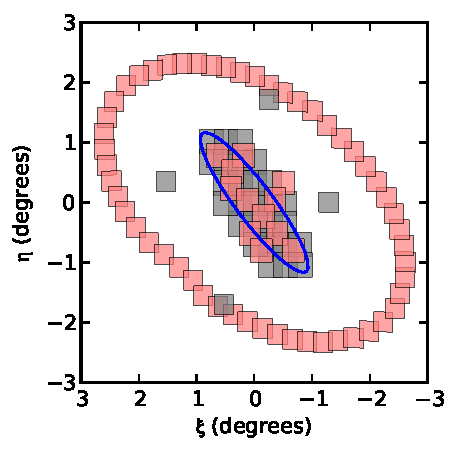
\includegraphics[height=8in]{figs/fieldmap.pdf}
%	\caption[WIRCam survey fields]{WIRCam survey fields in the 2007B (top) and 2009B (bottom) progammes. The fields are plotted on the INT/WFC star count map of \cite{Ibata:2005}.}
%	\label{fig:fieldmap}
%\end{figure}

%\begin{figure}[t]
%    \centering
%        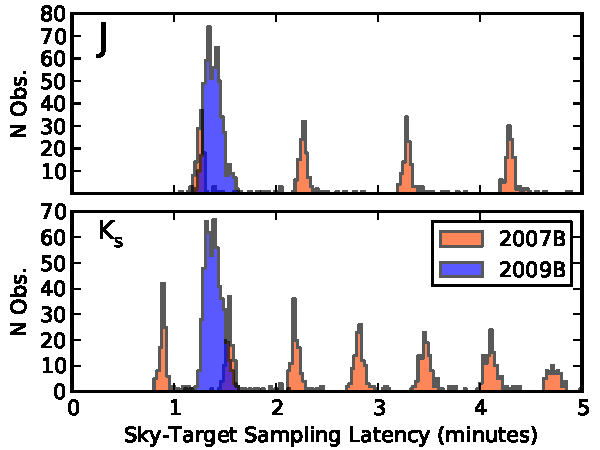
\includegraphics[width=\textwidth]{figs/sky_target_lag.pdf}
%    \caption{Time latency between target observations and sky sampling.}
%    \label{fig:sky_target_lag}
%\end{figure}

%\begin{figure}[t]
%    \centering
%        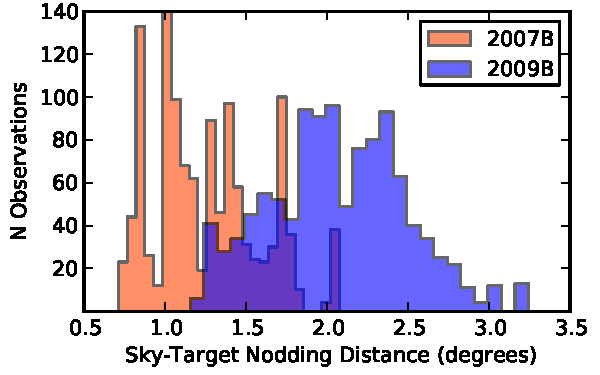
\includegraphics[width=\textwidth]{figs/sky_target_dist.pdf}
%    \caption{Distance between sky and target observations for 2007B and 2009B.}
%    \label{fig:sky_target_dist}
%\end{figure}

The initial survey was carried out in the 2007B semester by the CFHT Queue Service Observing under photometric conditions. As the observations were designed for resolved stellar analysis, we requested image quality (IQ) of 0.55\arcsec--0.65\arcsec, and our PSF modeling shows this was generally achieved (see Table \ref{tab:obssummary}). This programme covers M31 with 27 contiguous WIRCam fields covering the entirety of M31 out to the optical radius, $\mu_V=23$ mag arcsec$^{-2}$. The fields are arranged with at least 1\arcmin\ overlap in declination, and approximately 5\arcmin\ overlap in right ascension.
% FIXME check overlaps
With the dither pattern (see below), this arrangement yields a continuous mosaic that avoids masked pixels that obscure the eastern 3\arcmin\ of the WIRCam array. The field configuration is shown in Figure \ref{fig:fieldmap}.

Each field was integrated for $16\times 47 s = 12.5$ minutes in $J$ and $26\times 25 s = 10.8$ minutes in $K_s$. These integrations are sufficiently deep for resolved stellar photometry to reach at least 1 mag below the tip of the red giant branch, a crucial requirement for decomposing the contributions of red giant and asymptotic giant branch stars to the NIR light.

Our surface brightness analysis objective necessitated a regular monitoring of the sky's intensity. Since M31, with a $190\arcmin \times 60\arcmin$ optical disk, is much larger than the WIRCam fields of view, monitoring of the sky zeropoint is only possible by periodically pointing the telescope away from M31, towards blank sky---\emph{sky-target} (ST) nodding. The NIR sky intensity can be expected to change by 5\% in 10 minutes \citep{Adams:1996,Vaduvescu:2004}; since the sky itself is 5 dex brighter than the outer disk of M31 in the NIR, a 5\% uncertainty in the background would be fatal. To constrain the sky to within 1\%, we chose to monitor the sky so that at worst, a sky sample would be no more than 5 minutes removed from a M31 target image. Given the exposure times, this implied a sky (S)--target (T) observing sequence of $S^3T^8S^3$ in $J$ and $S^5T^{13}S^5$ in $K_s$.\footnote{Superscripts here denote the number of times an observation is repeated in sequence for a given target disk field.}

\section{2009B Semester}
\label{sec:obs9}

% Initial analysis of the 2007B data showed that sky subtraction suffered from roughly 6\% uncertainty in the sky level.
Although we had not developed yet sky offset optimization technology described in \S \ref{ch:dcoffset}, it was apparent that the 2007B data alone would not be sufficient for deep surface photometry of M31. Thus in our 2009B CFHT/WIRCam observing campaign, we set out to perform the \emph{most} exhaustive calibration of M31's NIR surface brightness that could be imagined with a CFHT/WIRCam-class instrument. Our programme was built upon the following axioms:

\begin{enumerate}
    \item \emph{Uncertainty from the temporal variability of the sky must be minimized.} No observation would be delayed by more than 1.5 minutes from a sky sample.
    \item \emph{Systematic uncertainty from the spatial structure of the NIR sky must be minimized.} By visiting many sky fields arranged about M31, we could average over the spatial structure in the sky.
    \item \emph{Uncertainties can be diminished by repeated trials.} Combining more images---each an independent estimate of the disk surface intensity---should reduce the statistical uncertainty of the mean surface intensity, and couplings between fields can be exploited to reduced systematic uncertainties.
    % \item \emph{Systematic sky offsets can be discovered by overlapping both disk and sky fields.}
\end{enumerate}

This reasoning lead to a 2009B observing campaign that included 12 fields on the disk of M31 with 40 repeated observations, integrating for 20 seconds in both the $J$ and $K_s$ bands (13.3 minutes/field/band integration, see Table \ref{tab:obssummary}). Temporal sky variations were minimized with an \emph{inefficient but necessary} ST$^2$S pattern (compared to 2007B: S$^3$T$^8$S$^3$ [$J$] and S$^5$T$^{13}$S$^5$ [$K_s$]). That is, each target observation was directly paired with a sky observation taken within 1.5 minutes (Fig. \ref{fig:sky_target_lag}). As shown in Figure \ref{fig:fieldmap}, each target field was overlapped with at least one other 2009B target field so that systematic uncertainties in surface intensities could be checked and corrected. Further, each 2007B disk field overlapped with at least one 2009B disk field so that a surface brightness distribution derived from the 2009B data could be directly used to calibrate the 2007B data.

Throughout the ST nodding pattern, the same sky field was never visited twice for the same target. Nods were semi-randomly assigned towards 53 sky fields, arranged in a ring removed at least 1\arcdeg\ from the optical radius of M31 (Fig. \ref{fig:fieldmap}). In order to maintain rapid telescope nods, only northern sky fields serviced the northern disk, and similar for the southern fields; the maximum offset on the sky was 3\arcdeg\ (see Fig. \ref{fig:sky_target_dist}). This random sampling of sky fields yielded two possible advantages: 1) when a median sky image is constructed, many \emph{sky shapes} are combined, possibly yielding an intrinsically flatter image of sky (see \S on median sky subtraction), and 2) if there is a coherent structure in the NIR sky, sampling fields of the sky degrees apart in rapid succession should average out these systematic biases in estimating the sky level \emph{on the disk}. Chapters \ref{ch:dcoffset} and \ref{ch:planarsky} discuss the veracity of these programme design hypotheses.

In their own right, the 2009B sky fields have considerable utility. Over the course of the the 2009B semester, each sky ring field was visited at least five times. Each visit adopted a position from the WIRCam DP5, five-point, dither pattern.\footnote{Implementing a program of random sky nods, while covering a dither pattern on each sky field, proved to be a challenge in the WIRCam phase two proposal interface.} The 100-second integration over each sky field allows deep source masks to be constructed for superior sky flat fielding and median sky subtraction. As an extension to the basic survey, the sky ring fields \texttt{01}, \texttt{13}, \texttt{27} and \texttt{39} were subjected to focussed integration sequences that document the sky variability at a stationary location on the sky over spans of 60--90 minutes. This study is discussed in \S \ref{sec:shapesurvey}. The 50 (45) minute integration in $J$ (and $K_s$) on these fields also allow deep colour magnitude diagrams to be constructed in the inner halo of M31 that complement the optical PAndAS survey \cite{Ibata:2007}.


% section Observations (end)

\section{Scalar Sky Optimization} % (fold)
\label{sec:scalarsky}

To improve upon this situation, each sky-subtracted image can be be taken as a independent estimate of the surface brightness at the pixels of M31 that the image covers. When taking a simple mean across all pixels to make a mosaic, as in the last chapter, artifacts arise because difference pixels are covered by different ensembles of images, creating field-to-field biases. This chapter will demonstrate how the couplings (overlaps) between images can allow these biases to be measured, and suppressed by introducing \emph{scalar sky subtraction offsets}.

The mathematical operation consists of using coupled image pairs $\vect{I}_i$ and $\vect{I}_j$. In their overlapping areas, one can construct the difference image $\vect{I}_i - \vect{I}_j$.
The goal is to drive such difference images to zero by introducing offsets, $\vect{\Delta}_i$, so that

\begin{equation}
    \langle (\vect{I}_i-\vect{\Delta}_i) - (\vect{I}_j-\vect{\Delta}_j) \rangle \rightarrow 0
    \label{eq:offsettheory}
\end{equation}

These image offsets can be thought of as subtle nudges of intensity applied to each image so that the overlapping network of images in a mosaic have a consistent surface brightness distribution. The role of the offsets is squarely to overcome the inaccuracy of classical NIR sky subtraction. This implies that the offsets we derive ought to be commensurate with the expected errors in sky-target nodding. That is, sky target nodding bestows a wide envelope of background uncertainty to each image; image coupling estimates where the image actually lies within that envelope. In \S \ref{sec:scalaranalysis}, I shall verify that this condition is met.


\subsection{Comparison to \sw{Montage}}
It should be noted that the \sw{Montage} software package \citep{Berriman:2008} already solves for coupled sky offsets as an integral phase of NIR mosaicing.\footnote{Another mosaicing software, \sw{Swarp} \citep{Bertin:2002}, offers to estimate the sky background from the surface of images themselves. This mode, of course, is unusable in such wide-field applications as M31.} \sw{Montage} identifies all overlapping pairs of images, and computes difference images of the overlapping pixels. In those difference images, the consistent astronomical structure is eliminated, producing a comparison of the pair's backgrounds. \sw{Montage} fits, in a least-squares sense, a constant level or a planar surface to each difference image. To yield a mosaic with consistent surface brightness structure, \sw{Montage} optimizes towards scalar (or surface) offsets for each image that minimize all difference images in accordance to the mathematical framework already described. The optimization algorithm is iterative: in each step the offset is solved for a given image that minimizes, in a least-squares sense, the difference images for that image given the existing offsets to its neighbours. This step is continued for each image in the mosaic, and is again iterated many times over until the solved offsets converge within a specified precision.

The use of \sw{Montage} to assemble a mosaic from the 2007B and 2009B WIRCam surveys has at least two major limitations: i) there is no account for propagated errors nor guarantee that the offsets yield a scientifically rigorous result, and ii) the iterative least-squares algorithm converges poorly with massive data sets. Indeed, the combined 2007B and 2009B data sets consist of 3924 $J$ and 4972 $K_s$ image frames that cover the disk of M31.

\subsection{Hierarchical offset optimization}
\label{sec:hierarchicaloffsets}

The shortcomings of \sw{Montage} for this extreme application of NIR mosaic construction motivate the development of a new procedure for solving the system of scalar sky offsets that correct the levels of WIRCam images to produce a continuous NIR mosaic of M31. Embedded in this procedure is an account of sky offset distributions, so that the statistical validity of the final mosaic can be assessed.

Solving sky offsets in the \sw{Montage} fashion---minimizing the difference in intensity between all overlapping pairs of images---is an optimization with a dimensionality that equals the number of frames. Clearly the 3924- and 4972-dimension optimizations over the WIRCam $J$ and $K_s$ data sets are not technically feasible. A revised sky offset optimization algorithm must seek to reduce the dimensionality of the data set.

A natural solution is to take advantage of the spatial organization of the WIRCam surveys. The 2007B and 2009B WIRCam surveys observed a total of 39 \emph{fields} across the M31 disk (illustrated in Figure \ref{fig:fieldmap}). Each WIRCam field is imaged with four detectors, arranged in a $2\times 2$ grid. Let us define a \emph{detector field} as the collection of images that are taken with a given detector, at a given field. Images in a detector field have the greatly simplifying property of all overlapping across a dominant section of the image frame. This means that images in a detector field can be straightforwardly combined to produce a \emph{detector field stack}. The construction of image stacks is described in \S\ref{sec:intradet}.

Next, the four detector field stacks within each field can be fitted into a \emph{block}. A block is a fundamental unit of the mosaic, as all images that are combined within a block were observed under contemporaneous sky conditions.

Finally, the blocks can be fitted into a galaxy-wide mosaic. This final step relies upon the nonlinear optimization of sky offsets for each of the 39 blocks in the combined 2007B and 2009B surveys. The solution to a 39-dimension optimization can be converged within a reasonable amount of computing. Section \ref{sec:interdet} describes the construction of blocks, and the fitting of blocks into mosaics. Key technologies for offset fitting included the computation of difference images between coupled images (presented in Appendix \ref{ch:diffimagemethod}), and a strategy to ensure that a global optimum is found in the minimization of image differences (Appendix \ref{cha:simplex}). Finally, the statistical properties of these mosaics is presented in \S\ref{sec:scalaranalysis}.

\section{Construction of detector field stacks}
\label{sec:intradet}

Scalar sky offsets are most easily computed between the images of a detector field, since individual image frames in a detector field share a common footprint. That is, each image in a detector field is an (approximately) independent random estimate of the true surface brightness of the detector field. The mean surface brightness in the stack of images on a detector field is taken as the best estimate of the actual surface brightness. For each image frame, the difference between the surface brightness of the image and its best-estimate surface brightness of the detector field is taken scalar offset that brings the image to the level of the detector field stack.

The best estimate surface brightness for each detector field stack is first estimated as the mean-combination of all images in a detector field stack.  Since the telescope dithers by a few arcminutes between individual integrations, the edges of the detector field stack have a surface brightness that is estimated from a subset of all the images in a stack. The smaller ensemble of images leads to a visible bias at the stack's edges compared to the middle, where all frames contribute to the surface brightness estimation.

A solution is to estimate offsets for each frame compared to this first detector field stack. Offsets are computed as the median of the difference image between the stack and individual image frames, as described in Appendix \ref{ch:diffimagemethod}. The original image frames, now with offsets applied, are re-combined into a detector field stack image. Now edge-effects are smaller. Nonetheless, offsets are estimated a second time to produce a finalized detector field stack image.

% --
% 
% Sky offsets are most easily computed at the first hierarchical level of the mosaic, a detector field, because all images sample the same area of the galaxy. Thus the mean surface brightness of the stack of frames in a detector field is the \emph{best estimate} of the surface brightness across the detector field's area. But simply making a mean-coaddition of frames in a detector field in unacceptable: the edges of the detector stack will be a subsample of the image ensemble, thus being visibly biased compared to the stack's centre. Instead, one wants to compute the offsets that can bring all frames to a common surface brightness level, and then coadd the offset frames.
% 
% \subsection{Procedure}
% 
% To construct detector stacks, we work from the resampled images and their weightmaps, described in \S \ref{ch:diffimagemethod}. Resampled images (which have a common scale, coordinate frame, and reference pixel (\texttt{CRVAL} coordinate) allow overlapping areas of pixels to be directly compared using the procedures in \S \ref{ch:diffimagemethod}.
% 
% As a first pass, the resampled frames are average-combined using \sw{Swarp}. The centre of the combined frame will represent the best estimate of the mean surface intensity of the detector field, while the edges will be biased, as discussed. An initial scalar sky offset of each individual frame to the mean surface intensity is estimated by taking the median of the difference image of that frame to the average-combined image. The difference images are biased at the edges, so that sky offsets still need to be refined. As a second iteration the levels of the individual frames are offset by the amount of it's initial offset hose. Those offset frames are then average-combined, again with Swarp. The result is a much cleaner combined image. The sky offsets are again estimated from the difference of an individual frame to the combined image. With these refined offsets, the averaged-combined stack is again made, for a third, and final, time.
% 
% These stacks now become the fundamental units of assembling an all-galaxy mosaic in \ref{sec:interdet}

\subsection{Dispersion of surface intensity estimates within a detector field stack}

%\begin{figure}[p]
%    \centering
%        \includegraphics[width=\textwidth]{figs/stack_sigma_dist.pdf}
%    \caption[Detector field stack dispersions, $\sigma_s$]{Detector field stack dispersions, $\sigma_s$, for the $J$ (top) and ($K_s$) bands.}
%    \label{fig:sigma_stack}
    % disksky/stack_sigma_plot.py
%\end{figure}

% \begin{figure}[t]
%     \centering
%         \includegraphics[height=4in]{figs/stack_offset_dist.pdf}
%     \caption{Distribution of sky offsets within detector field stacks.}
%     \label{fig:stackoffsetdist}
% \end{figure}

If $\Delta_i$ is the scalar sky offset that adjusts frame $i$ to the mean level of the stack, then we may define the dispersion (sample standard deviation) of these offsets as $\sigma_s$, the stack dispersion.
% 
% \begin{equation}
%     \sigma_s^2 = \frac{1}{n_I - 1}\sum_i \Delta_i^2,
% \end{equation}
% 
% \noindent for $n_I$ images in a detector field stack. 
This stack dispersion is effectively the uncertainty in the level of a detector field stack. Figure \ref{fig:sigma_stack} shows the distribution of $\sigma_s$ for both $J$ and $K_s$ bands in the 2007B and 2009B semesters across all detector field stacks. The stack dispersion of $J$ band fields is roughly half that in the $K_s$ band---commensurate with the smaller sky amplitude in $J$ than $K_s$. Surprisingly, the levels of 2009B detector field stacks are no better constrained than 2007B. This suggests that rapid sky-target nodding with a frequency of 1.2 minutes \emph{does not} decrease the uncertainty in sky level at the target compared to sky sampling on 5 minute frequencies. Rather, simply nodding the telescope on scales of 1\arcdeg--3\arcdeg\ is a significant source of sky level uncertainty. This is commented upon further in \S \ref{sec:strategydiscussion} and Fig \ref{fig:offsets_stationarysky}.

\subsection{Pixel RMS of detector field stacks}

Each area of the M31 disk is covered by at least one detector field stack. Although these stacks are subjected to $\sigma_s$ systematic intensity uncertainty, each pixel has a random intensity uncertainty governed by Poisson statistics. Such noise can be measured empirically from the pixel standard deviation of stack images that have been cleaned of sources, and background subtracted; the \sw{Source Extractor} package \citep{Bertin:1996} provides such `background RMS' maps. Figure \ref{fig:rmsshape} shows the horizontal trend of pixel noise across representative detector stack images for the $J$ and $K_s$ bands in the 2007B and 2009B semesters.

%\begin{figure}[p]
%	\centering
%		\includegraphics[width=\textwidth]{figs/rmsshape.pdf}
%	\caption[Trends of pixel RMS noise across $J$ and $K_s$ detector stacks]{Trends of pixel RMS noise across $J$ (top) and $K_s$ detector stacks, for 2007B (red) and and 2009B (blue) semesters.}
%	\label{fig:rmsshape}
%\end{figure}

The 2009B data do not provide any reduction is pixel noise compared to 2007B. The mean pixel noise in the $J$ band is $1.1\times 10^{-10}$ ADU s$^{-1}$ pix$^{-2}$, and $4.0\times10^{-10}$ ADU s$^{-1}$ pix$^{-2}$ in $K_s$ stacks. Noise is uniform across the stack frame, save for the peripheral 2\arcmin, where the dither pattern provides less coverage. In all cases, pixel noise does appears to increase  $\sim 3\times$ towards the stack edge.
% This suggests that weight maps should be constructed from pixel RMS maps both for mosaic construction (FIXME currently they are not!), and image coupling. Indeed, the image coupling algorithms presented in \S \ref{sec:interdet} are heavily reliant upon these low $S/N$ regions of the stacks to ensure intensity continuity across stack images in the mosaic. TODO: need to use RMS-derived weight maps when computing image differences.

\section{Optimization of inter-field sky offsets}
\label{sec:interdet}

The detector field stacking phase (\S \ref{sec:intradet}) created high-\sn\ mosaics of the region covered by a given WIRCam detector at each survey field. Although these detector stacks are best estimates of the galaxy surface intensity at their regions, I showed in the previous section that these detector stacks have systematic sky surface intensity uncertainties of $\sigma_s$. In this section, it is my goal to further diminish sky subtraction uncertainty by leveraging the information in the couplings between adjacent detector fields to piece together a consistent wide-field mosaic. \emph{If} we assume that the detector stacks are flat, with respect to their sky error, solving for the sky offsets that minimize the difference in intensity between overlapping images will naturally provide a strong correction on the residual sky error in each detector stack.

Our primary desiderata for assembling the galaxy-wide mosaic is

\begin{enumerate}
    \item a record of each coupling between pairs of detector fields, and
    \item for each coupled image pair, a best estimate of their difference in intensity in the overlapping area: $\langle \vect{I}_i-\vect{I}_j \rangle$, and its uncertainty $\sigma_{\Delta ij}$.
\end{enumerate}

\noindent Appendix \ref{ch:diffimagemethod} describes how this image coupling information is reduced.

In the spirit of Eq \ref{eq:offsettheory}, our task is reduced to solving the scalar sky offsets $\Delta_i$ that minimize the difference in intensity between detector stacks.
% \footnote{Note that I also assume the use of \emph{scalar} sky offsets, whereby sky errors are simply in the level of the field, and that sky errors do not possess a shape across a detector field. This is to reduce the dimensionality of the optimization problem. The technique could nonetheless be extended to 2D sky offsets if the problem requires.}
Since the detector stacking phase has already reduced the degrees of freedom in the mosaic by over an order of magnitude, the iterative sky offset algorithm used by \sw{Montage} is feasible. Instead, I approach the problem from the more flexible framework of multidimensional optimization.

Let us define the objective function that encapsulates the effect of scalar sky offsets on reducing the intensity difference between coupled images:

\begin{equation}
    \mathcal{F} \left(\Delta_1,\ldots,\Delta_n \right) = \sum_{i,j} \mathcal{W}_{ij} \left( \langle \vect{I}_i - \vect{I}_j \rangle - \Delta_i + \Delta_j \right)^2,
    \label{eq:objf}
\end{equation}

\noindent which we intend to minimize by finding the optimal set of scalar sky offsets $\Delta_i$ for each of the detector fields $i$. Note that each coupled image pair is its own term in the objective summation, and that there are as many degrees of freedom ($\Delta_i$) as there are images in the mosaic. Each coupling is tempered by a weighting term $\mathcal{W}_{ij}$:

\begin{equation}
    \mathcal{W}_{ij} = \frac{A_{ij}}{\sigma_{\mathrm{\Delta ij}}},
\end{equation}

\noindent so that more priority is given to couplings of larger areas ($A_{ij}$), and small standard deviations of their difference images ($\sigma_{\Delta ij}$).

Note that the objective function in Eq \ref{eq:objf} puts no constraint on the net sky offset: $\sum \Delta_i$. Assuming that sky subtraction errors are normally distributed, and not biased, sky subtraction offsets should not add a net amount of flux to the mosaic. Fortunately, it is possible to impose this constraint \textit{post facto} by subtracting the mean offset from the sky offsets:

\begin{equation}
    \Delta_i^* = \Delta_i - n^{-1}\sum_{j=1}^n \Delta_j.
    \label{eq:netzero}
\end{equation}

Given the image coupling records, I optimize the set of $\Delta_i$ using the \cite{Nelder:1965} (NM) downhill simplex algorithm. This NM algorithm has the advantage of being naturally multi-dimensional, and being able to work without knowledge of the gradient of the objective function. Instead, the NM algorithm operates by constructing a geometric simplex of $N+1$ dimensions that samples the sky offset parameter space. By evaluating the objective function at each vertex of the simplex, the NM algorithm adapts simplex's shape to ultimately contract upon a minimum.

But NM has two weaknesses. First, it is a \emph{greedy} optimizer that will converge into any local minimum, without necessarily seeking the global minimum. Second, for high-dimension optimizations (many fields in the mosaic), the NM may fail to converge in a reasonable number of objective function evaluations \citep{Neumann:2006}. Without solving these issues, a minimization of Eq \ref{eq:objf} with an off-the-shelf NM code yields a mosaic with obvious discontinuities across fields. To solve the first problem, I develop a Multi-Start Reconverging NM (MSRNM) downhill simplex driver in Appendix \ref{cha:simplex}. This algorithm allows the NM to cumulatively cover a larger portion of parameter space to probabilistically ensure convergence into a global optimum.

Abating the second issue, of NM's failure on high-dimension problems, is more straightforward. Consider that an all-M31 WIRCam mosaic, using both the 07B and 09B detector stacks in a given band, will be composed of
% 4 (27 + 12)=156
156 detector stacks. Rather than immediately optimizing over a 156--dimensional space, we extend the pattern of hierarchy to optimize the sky offsets within blocks. First discussed in \S\ref{sec:hierarchicaloffsets}, these blocks are built from the $2\times 2$ array of detector field stacks that cover a given WIRCam field. Offsets between the 39 blocks are then optimized to create a galaxy-wide mosaic. In detail, the optimization of the scalar sky-fitted WIRCam mosaics proceeds as followings:

\begin{enumerate}
    \item\label{ls:blockopt} For each block of four detector stacks, a block mosaic is formed. Sky offsets for the detector stacks are solved with the objective function (Eq \ref{eq:objf}), and those offsets are treated with Eq \ref{eq:netzero}. Using these scalar sky offsets, the adjusted detector stacks are combined with \sw{Swarp} to make a block mosaic.
    
    With respect to the MSRNM algorithm (Appendix \ref{cha:simplex}), the downhill simplex is started $N_s=100N_d=400$ times. Sky offsets in the initial simplex have a normal dispersion of $5\times10^{-11}$ ADU s$^{-1}$ pix$^{-2}$, and the converged point is inflated with a restart dispersion of $1\times10^{-11}$ ADU s$^{-1}$ pix$^{-2}$.
    
    \item\label{ls:mosaicopt} The collection of blocks is then assembled into a galaxy-wide mosaic by solving for scalar sky offsets between the block mosaics. Here the downhill simplex is started $N_s=10N_d=390$ times. The sky offsets in the initial simplex have a dispersion of $5\times10^{-9}$ ADU s$^{-1}$ pix$^{-2}$, and the converged point is inflated with a restart dispersion of $1\times10^{-10}$ ADU s$^{-1}$ pix$^{-2}$.

% I implement this by retaining the coupling information (\ie, $\langle \vect{I}_i-\vect{I}_j \rangle$) of the detector stacks rather than computing new coupling information between the field block mosaics. To do so, I adjust each detector field image difference by the sky offset computed in Step 1. Then, when computing the objective function, the $\Delta_i$ is fixed across all detector fields in a block, so that the entire field block is offset in unison.
% Rather than computing the couplings between blocks, the coupling information between 
\end{enumerate}

\section{Analysis of scalar-sky fitted mosaics}
\label{sec:scalaranalysis}

%\begin{figure}[p]
%    \centering
%        \includegraphics[height=7.75in]{figs/mosaicmaps_dc.png}
%    \caption[Scalar-sky fitted WIRCam $J$ and $K_s$ mosaics of M31]{Scalar-sky fitted WIRCam $J$ and $K_s$ mosaics of M31. Surface intensity is presented in ADU s$^{-1}$ pix$^{-2}$, calibrated against the 2MASS point source catalog (\S\ref{sec:photocal}), for each $0\farcs3\times0\farcs3$ WIRCam pixel.}
%    \label{fig:mosaicmaps_dc}
%\end{figure}

Mosaics constructed with scalar-sky fitting to both 2007B and 2009B detector stacks are shown in Figures \ref{fig:mosaicmaps_dc}. The eye is an adept tool for judging near-infrared mosaics, and these scalar-sky fitted mosaics are clearly more uniform than ones derived from immediate \iiwione\ pipeline products. Nonetheless, discontinuities in the outer disk hint at the limitations of scalar sky optimization. Across fields there are overall biases in sky level: the $J$ mosaic is over-subtracted across the minor axis, while the $K_s$ mosaic shows under-subtraction in the vicinity of NGC 205, and a peculiar gradient at the southwest mosaic edge.
% The $J$ mosaic is more uniform than the $K_s$ image, commensurate with the smaller amplitude of sky and its variations in the $J$ band.

% \begin{figure}[t]
%     \centering
%         \includegraphics[width=\textwidth]{figs/intra_offset_dist.pdf}
%     \caption[Intra-block scalar sky offset distribution]{Scalar sky offsets that match levels of detector stacks within a block of four detector fields (a WIRCam field).}
%     \label{fig:intra_offset_dist}
%     % intrafielddcskyoffsetdist.py
% \end{figure}

%\begin{figure}[p]
%    \centering
%        \includegraphics[height=7.5in]{figs/dc/offset_hierarchy.pdf}
%    \caption[Distributions of scalar sky offsets in the three hierarchical stages of sky fitting]{Distributions of scalar sky offsets in the three hierarchical stages of sky fitting: (1--top) fitting WIRCam frames into detector field stacks;  (2--middle) fitting detector field stacks into blocks; (3--bottom) fitting stacks--in blocks--to other blocks in the mosaic.}
%    \label{fig:offset_hierarchy}
    % offset_hierarchy.py
%\end{figure}

\begin{table}[t]
    \centering
    \caption[Hierarchy of scalar sky offsets]{Hierarchy of scalar sky offsets. The `Total' sky offsets track the net offset of individual WIRCam image frames into the fitted mosaic. $\langle I_\mathrm{sky}\rangle$ is taken as the median sky surface intensity observed in the entire data set: $1.0\times 10^{-7}$ and $4.3\times 10^{-7}$ ADU s$^{-1}$ pix$^{-2}$ in the $J$ and $K_s$ bands, respectively.}
    \label{tab:offset_hierarchy}
\begin{tabular}{ll|ll|ll}
% \hline
 &  & \multicolumn{2}{c|}{$J$} & \multicolumn{2}{c}{$K_s$} \\ % \cline{3-4} \cline{5-6}
% \hline
Offset Type & Sem. & $\sigma_\Delta$ & $\frac{\sigma_\Delta}{\langle I_\mathrm{sky}\rangle }$ & $\sigma_\Delta$ & $\frac{\sigma_\Delta}{\langle I_\mathrm{sky}\rangle }$ \\
 & & \tiny{(ADU s$^{-1}$ pix$^{-2}$)} &  \tiny{(\%)} & \tiny{(ADU s$^{-1}$ pix$^{-2}$)} &  \tiny{(\%)} \\
\hline
\multirow{2}{*}{Frame to stack} & 07B & $8.6\times 10^{-10}$ & 0.86 & $5.4\times 10^{-9}$ & 1.26\\
% \hline
 & 09B  & $6.3\times 10^{-10}$ & 0.63 & $4.8\times 10^{-9}$ & 1.12\\
\hline
\multirow{2}{*}{Stack to block} & 07B & $6.0\times 10^{-11}$ & 0.06 & $2.9\times 10^{-10}$ & 0.07\\
% \hline
  & 09B & $2.4\times 10^{-11}$ & 0.02 & $1.5\times 10^{-10}$ & 0.03\\
\hline
\multirow{2}{*}{Stack to mosaic} & 07B & $4.5\times 10^{-10}$ & 0.45 & $2.3\times 10^{-9}$ & 0.53\\
% \hline
  & 09B & $2.4\times 10^{-10}$ & 0.24 & $1.9\times 10^{-9}$ & 0.44\\
% \hline
\hline
\multirow{2}{*}{Total} & 07B & $9.7\times 10^{-10}$ & 0.97 & $5.8\times 10^{-9}$ & 1.35 \\
% \hline
  & 09B & $6.7\times 10^{-10}$ & 0.67 & $5.1\times 10^{-9}$ & 1.19 \\
% \hline
\end{tabular}

% Total offsets derived from offset_hierarchy.py's computeTotalSkyOffsetDist
% Total offsets for 2007B J: sigma= 9.67e-10 ADU/s/pix
% Total offsets for 2009B J: sigma= 6.74e-10 ADU/s/pix
% Total offsets for 2007B Ks: sigma= 5.82e-09 ADU/s/pix
% Total offsets for 2009B Ks: sigma= 5.14e-09 ADU/s/pix

\end{table}

\begin{table}[t]
	\centering
	\caption[Coupled block differences and residual differences after
	scalar sky offsets]{Coupled block intensity differences and residual intensity differences after application of scalar sky offsets: 25th, 50th and 75th percentiles of distribution. Differences are presented as a percent of the typical sky level (see caption of Table \ref{tab:offset_hierarchy}).}
	\label{tab:resid_diffs}
	\begin{tabular}{lccc}
		& \multicolumn{3}{c}{Coupled Block $\langle I_i - I_j\rangle / \langle I_\mathrm{sky} \rangle$ (\%)} \\
		& 25th & 50th & 75th \\
		\hline
		$J$, uncorrected & 0.18 & 0.35 & 0.67 \\
		$J$, scalar offset & 0.01 & 0.03 & 0.06 \\
		\hline
		$K_s$, uncorrected & 0.21 & 0.46 & 0.81 \\
		$K_s$, scalar offset & 0.01 & 0.02 & 0.05 \\
		\hline
	\end{tabular}
\end{table}

% Output from thesis/residualsky.py
% Diffs
% J
% 0.181256551435
% 25th 1.81e-01
% 50th 3.48e-01
% 75th 6.70e-01
% Ks
% 0.212691318046
% 25th 2.13e-01
% 50th 4.62e-01
% 75th 8.09e-01
% --
% Residual Diffs
% J
% 0.0104902501307
% 25th 1.05e-02
% 50th 2.82e-02
% 75th 6.44e-02
% Ks
% 0.00969165035535
% 25th 9.69e-03
% 50th 2.42e-02
% 75th 4.96e-02


\paragraph{Amplitudes of scalar sky offsets.} The distribution of scalar sky offsets provide an excellent characterization of sky subtraction uncertainties when using sky-target nodding. Recall that sky offsets are optimized hierarchically: WIRCam frames are fitted to stacks, stacks are fitted into blocks of four contemporaneously-observed WIRCam detector fields, and these blocks are fitted into a mosaic. Figure \ref{fig:offset_hierarchy} shows the distributions of sky offsets at each stage of optimization, with an implicit comparison between the 2007B and 2009B programs. Table \ref{tab:offset_hierarchy} lists the standard deviations of these offset distributions with respect to the typical sky level observed in the $J$ and $K_s$ bands.

Sky glow tends to be $\sim 4\times$ greater in the $K_s$ band than $J$ in calibrated flux units.
% Sky offsets, then, are also commensurately larger in $K_s$ than $J$.
Yet even relative to the typical sky level, $K_s$ sky offsets are larger than $J$ offsets, indicating that the $K_s$ sky has greater contrast in its sky glow structures.

Within the hierarchy of sky fitting, simply fitting frames to a stack is most significant: a correction on the order of 1\% of the sky intensity. Fitting these stacks into a mosaic is a further $\sim 0.5\%$ correction. The offsets to fit a stack into a block of four detector field stacks are smallest: 0.01\% of the sky level. This suggests that on the scale of the $2\times 2$ WIRCam array, the contemporaneously-observed images from each detector are subject to roughly the same sky biases.

A comparison between the net sky offsets applied to the 2007B and 2009B data sets is provocative. The net uncertainty in sky level due to sky-target nodding, as measured by the total sky offset applied to each frame, decreased by 30\% and 12\% in the 2009B $J$ and $K_s$ data sets, respectively. The performance of the two observational strategies will be further discussed in \S \ref{sec:strategydiscussion}.

% In Figure \ref{fig:intra_offset_dist}, I show the distribution of offsets within these blocks of four detector fields. The $J$ data has $5\times$ smaller offsets within a block then $K_s$; which makes sense given the overall amplitudes of sky changes. But the 09 data seems to have 2--3$\times$ smaller intra-block offsets. This is not seen in the distribution of $\sigma_s$ (Figure \ref{fig:sigma_stack}), but $\sigma_s$ is more a test of the inherent variation of the sky in time and space, which 09 never could overcome. But 09 had deeper sampling of each field, which is turn can give it a best estimate of the mean surface intensity of each stack.
% 
% In Figure TODO %\ref{fig:inter_offset_dist}
% I similarly plot the distribution of scalar sky offsets between blocks in both the $J$ and $K_s$ mosaics. Scalar sky offsets \emph{between} blocks are FIXME orders of magnitude larger than sky offsets \emph{within} blocks. This demonstrates that although the detector field stacks within a block are built from completely independent sets of sky flats and median sky frames, the very fact these data are imaged contemporaneously under the same sky conditions causes their sky biases to be similar. Sky offsets are mandated by natural sky uncertainties, not data reduction failures.

\paragraph{Statistical acceptability of scalar sky offsets.} Recall that scalar sky offsets were initially introduced as nudges in intensity to overcome uncertainty in the sky level of detector field stacks. Within the framework of hierarchical sky offset optimization, the smallest detector field stack dispersion within each block---$\min(\sigma_{s,\mathrm{block}})$---represents the lower limit uncertainty in the intensity level of a block. If sky offsets fitted between blocks are statistically permissible, then $\Delta_\mathrm{sky,block} \lesssim \min (\sigma_{s,\mathrm{block}})$. In figure \ref{fig:offset_sigmastack}, I plot a field map (in the same spatial configuration as Fig \ref{fig:fieldmap}) painted with the values of $\Delta_\mathrm{sky,block} / \min (\sigma_{s,\mathrm{block}})$ for each detector field in the $J$ and $K_s$ mosaics. The sky offsets are indeed distributed within the uncertainty budgeted by $\min (\sigma_{s,\mathrm{block}})$: the sky offsets are statistically acceptable.

% \begin{figure}[t]
%   \centering
%   \includegraphics[width=\textwidth]{figs/dc/J0709_offset_sigmastack.pdf}
%   \caption{Acceptability of $J$ scalar sky sky offsets: ratio of $\Delta_\mathrm{sky}/\sigma_s$.}
%   \label{fig:J0709_offset_sigmastack}
% \end{figure}
% 
% \begin{figure}[t]
%   \centering
%   \includegraphics[width=\textwidth]{figs/dc/K0709_offset_sigmastack.pdf}
%   \caption{Acceptability of $K_s$ scalar sky sky offsets: ratio of $\Delta_\mathrm{sky}/\sigma_s$.}
%   \label{fig:K0709_offset_sigmastack}
% \end{figure}

%\begin{figure}[t]
%    \centering
%        \includegraphics[width=\textwidth]{figs/dc/offset_sigmastack.pdf}
%    \caption[Acceptability of $J$ and $K_s$ scalar sky offsets between blocks, as measured by the ratio of $\Delta_\mathrm{sky}/\sigma_s$]{Acceptability of $J$ (top) and $K_s$ (bottom) scalar sky offsets between blocks, as measured by the ratio of $\Delta_\mathrm{sky}/\sigma_s$.}
%    \label{fig:offset_sigmastack}
%\end{figure}


\paragraph{Residual image level differences.} Although the scalar sky offsets are statistically valid, they are not perfect prescriptions against the sky subtraction uncertainties of each image stack---that much is visually true. A measure of the limitation of sky offset fitting are the residual image level differences between coupled fields, $(\vect{I}_i - \Delta_i) - (\vect{I}_j - \Delta_j)$, after the sky offsets $\Delta_i$ have been optimally fitted.

Table \ref{tab:resid_diffs} shows the distributions of both image level differences between coupled blocks, and residual differences after application of scalar sky offsets. Uncorrected, the ensemble of coupled blocks have a median intensity difference of $\sim 0.4\%$ of the typical sky background intensity. Scalar sky offsets decrease the differences between overlapping fields to $\sim 0.02\%$.

Figures \ref{fig:J0709B_net_resid} and \ref{fig:K0709B_net_resid} show networks of residual image differences as a percentage of local surface intensity in the $J$ and $K_s$ mosaics. This visualization mimics the spatial distribution of the 2007B and 2009B WIRCam fields (Fig \ref{fig:fieldmap}), but the field boxes have been exploded to allow room for lines to connect coupled detector fields. The thickness and colour of the line is modulated against the size of the residual image difference compared to the local surface intensity in the image overlap region. Where disk \sn\ is high in the inner M31 disk, the residual image differences are $\lesssim 1\%$ of the local surface intensity. But in the outer disk, residual image differences can become formidable: 50\%--100\% of the local surface intensity.

Of course, it is precisely this residual image level difference that was sought to be minimized as part of the optimization's objective function (Eq \ref{eq:objf}). The inability of scalar sky offset optimization to eliminate residual image differences should not be interpreted as a failure to detect the global minimum; the MSRNM optimization algorithm appears robust in arriving at this offset solution set. The correct interpretation is that sky uncertainties are not entirely scalar on the scale of WIRCam fields: there are residual sky shapes associated with each field that make 1\% intensity continuity in the outer M31 disk impossible with a purely scalar error parameterization.

%\begin{figure}[p]
%	\centering
%		\includegraphics[width=\textwidth]{figs/dc/J0709B_net_resid.pdf}
%	\caption[Residual intensity difference network in $J$]{Percent residual intensity differences (relative to local surface intensity) between coupled fields in the $J$ scalar sky optimization with both 2007B and 2009B data sets.}
%	\label{fig:J0709B_net_resid}
%\end{figure}

%\begin{figure}[p]
%	\centering
%		\includegraphics[width=\textwidth]{figs/dc/K0709_net_resid.pdf}
%	\caption[Residual intensity difference network in $K_s$]{Percent residual intensity differences (relative to local surface intensity) between coupled fields in the $K_s$ scalar sky optimization with both 2007B and 2009B data sets.}
%	\label{fig:K0709B_net_resid}
%\end{figure}

\paragraph{Residual sky shape uncertainties in detector field stacks.}

%\begin{figure}[t]
%    \centering
%        \includegraphics[width=\textwidth]{figs/slices_137.pdf}
%    \caption[Horizontal slices across the $J$ and $K_s$ mosaics at $\eta=1.1$]{Horizontal slices across the $J$ (top) and $K_s$ (bottom) mosaics at $\eta=1.1$ (see green slice band on inset field map). The black line is the mosaic surface intensity, while the coloured bands are surface intensities of individual blocks.}
%    \label{fig:slices_137}
%\end{figure}

The role of residual sky shape uncertainties in the mosaic can be seen by analyzing the profiles of individual detector field stacks across the mosaic, and the discontinuities of these profiles between stacks. Figure \ref{fig:slices_137} shows a 0.1\arcdeg -wide horizontal slice through the $K_s$ mosaic across the northern fields, where the M31 surface intensity is low. Not only does this slice show the profile of the median mosaic (black), but is also decomposed into slices through the individual blocks that are composited into the mosaic. Now the source of the residual difference image flux is clear: blocks do not necessarily have continuous shapes. Scalar sky offsets will never produce a perfectly fitting mosaic, as each block has a \emph{residual sky shape} due to the sky fields observingly different shapes of sky structures than the disk observations.

The anecdotal case of Fig \ref{fig:slices_137} demonstrates that $J$ band detector field stacks have modest shape discontinuities, which is borne out by the visual appearance of the $J$ mosaic compared to $K_s$. At the surface brightness of this outer disk field, $\mu_{K_s}\sim 20$ mag arcsec$^{-2}$, residual sky flux can erase, and even reverse, the intrinsic shape of the disk (\eg, M31-1 and M31-3 in the $K_s$ slice of Fig \ref{fig:slices_137}).

Fields M31-3 and M31-7 have slight shape mis-matches in Fig. \ref{fig:slices_137}, but do show large disagreement in level. In the $K_s$ mosaic, $\eta$-axis (North-South) slope discontinuities yield a nearly 100\% disagreement in the level between fields M31-3 and M31-7.

Ultimately, the only remedy for this problem is to optimize against the shape---not just level---of the residual sky in each mosaic block. An attempt at just that is described in Ch \ref{ch:planarsky}.

% section scalarsky (end)

\bibliography{master}

\end{document}
